\documentclass[letterpaper,11pt]{article}
\oddsidemargin -1.0cm \textwidth 17.5cm

\usepackage[utf8]{inputenc}
\usepackage[activeacute,spanish, es-lcroman]{babel}
\decimalpoint
\usepackage{amsfonts,setspace}
\usepackage{amsmath}
\usepackage{amssymb, amsmath, amsthm}
\usepackage{comment}
\usepackage{float}
\usepackage{amssymb}
\usepackage{dsfont}
\usepackage{anysize}
\usepackage{multicol}
\usepackage{enumerate}
\usepackage{graphicx}
\usepackage[left=1.5cm,top=2cm,right=1.5cm, bottom=1.7cm]{geometry}
\setlength\headheight{1.5em} 
\usepackage{fancyhdr}
\usepackage{multicol}
\usepackage{hyperref}
\usepackage{wrapfig}
\usepackage{subcaption}
\usepackage{siunitx}
\usepackage{cancel}
\usepackage{mdwlist}
\usepackage{svg}
\pagestyle{fancy}
\fancyhf{}
\renewcommand{\labelenumi}{\normalsize\bfseries P\arabic{enumi}.}
\renewcommand{\labelenumii}{\normalsize\bfseries (\alph{enumii})}
\renewcommand{\labelenumiii}{\normalsize\bfseries \roman{enumiii})}


\begin{document}

\fancyhead[L]{\itshape{Facultad de Ciencias F\'isicas y Matem\'aticas}}
\fancyhead[R]{\itshape{Universidad de Chile}}
\rfoot[]{pág. \thepage}

\begin{minipage}{11.5cm}
    \begin{flushleft}
        \hspace*{-0.6cm}\textbf{FI1000 Introducción a la Física Clásica}\\
        \hspace*{-0.6cm}\textbf{Tutor:} Alejandro Cartes
    \end{flushleft}
\end{minipage}

\begin{picture}(2,3)
    \put(366, -10){
\includegraphics[scale=0.9]{2020-1/Imágenes/logo/dfi-fcfm.pdf}}
\end{picture}

\begin{center}
	\LARGE\textbf{Tutoría Crec}
\end{center}

\vspace{-1cm}
\begin{enumerate}\setlength{\itemsep}{0.4cm}

\item[]

\item \textbf{[Mov. Relativo]} Un piloto debe viajar hacia el este desde $A$ hasta $B$ y luego regresa de nuevo a $A$ hacia el oeste. La velocidad del aeroplano en el aire es $\mathbf{v}$ y la velocidad del aire con respecto al suelo es $\mathbf{u}$. La distancia entre $A$ y $B$ es $l$ y la velocidad del aeroplano en el aire es constante.
    \begin{enumerate}
        \item Si $u=0$ (aire quieto), demuestre que el tiempo del viaje redondo es $t_0 = 2l/v$

        \item \label{b} Suponga que la velocidad del aire va hacia el este (u oeste). Demuestre que el tiempo del viaje redondo es, entonces, $t_E = t_0 / (1 - u^2/v^2)$

        \item \label{c} Suponga que la velocidad del aire es hacia el norte (o hacia el sur). Demuestre que el tiempo del viaje redondo es, entonces, $t_N = t_0 / \sqrt{1 - u^2/v^2}$

        \item En las partes P\ref{b} y P\ref{c}, ¿debemos suponer que $u<v$? ¿Por qué?
    \end{enumerate}

\begin{minipage}{0.7\linewidth}
    \item \textbf{[Mov. Circular + Energía]}  Un esquiador de masa $m$ realiza un salto durante los Juegos Olímpicos de Invierno en la pista mostrada en la figura, partiendo del reposo. Despreciando cualquier roce entre las superficies y con el aire:
    
    \begin{enumerate}
        \item Encuentre la aceleración total del esquiador en el punto de despegue de la pista
    
        \item Determine la máxima altura que alcanza luego de saltar
    \end{enumerate}
\end{minipage}
\hfill
\begin{minipage}{0.22\linewidth}
    \begin{figure}[H]
        \centering
        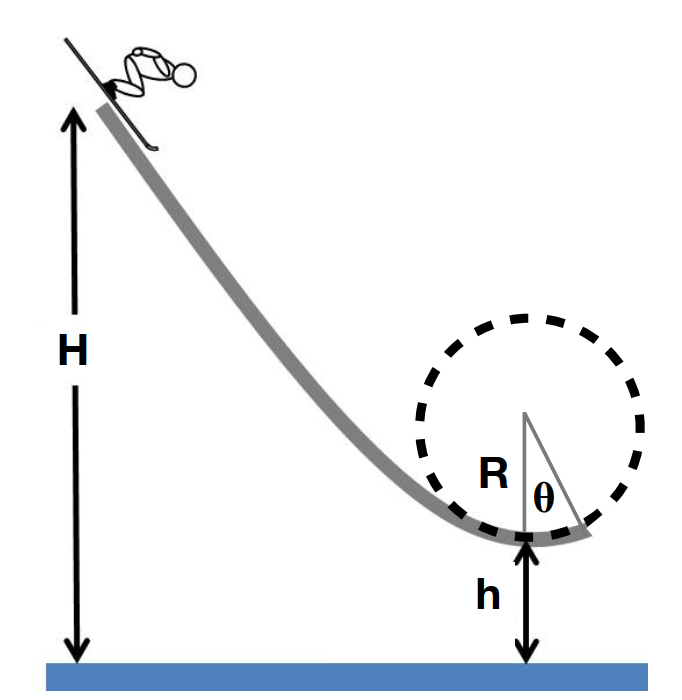
\includegraphics[width=1\linewidth]{tutorías/2023/img/ski.png}
    \end{figure}
\end{minipage}

\item \textbf{[Dinámica + Energía]} Una masa $m$ resbala, sin roce y debido a la gravedad, por la superficie de una semiesfera de radio $R$. La masa parte desde la cúspide sin velocidad inicial. Sea $P$ el punto en el cual la masa se separa de la semiesfera. Encuentre el ángulo de elevación $\theta_0$ del punto P.

\begin{figure}[h!]
    \centering
    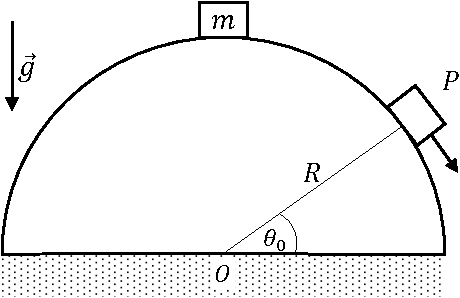
\includegraphics[scale=0.65]{2020-1/Imágenes/aux10/semiesfera_masa.pdf}
\end{figure}

% Para imágenes vectoriales -> el texto tiene que estar en LaTeX
% \begin{figure}[htbp]
%   \centering
%   \svgpath{../Imagenes/ejercicios}  -> .. irse pa'trás 
%   \includesvg{ej5.svg}
% \end{figure}

\end{enumerate}
\end{document}
